\talkslide{separate}{Putting it all together}{Timing: provisional}{Here is the full structure.}{
\centering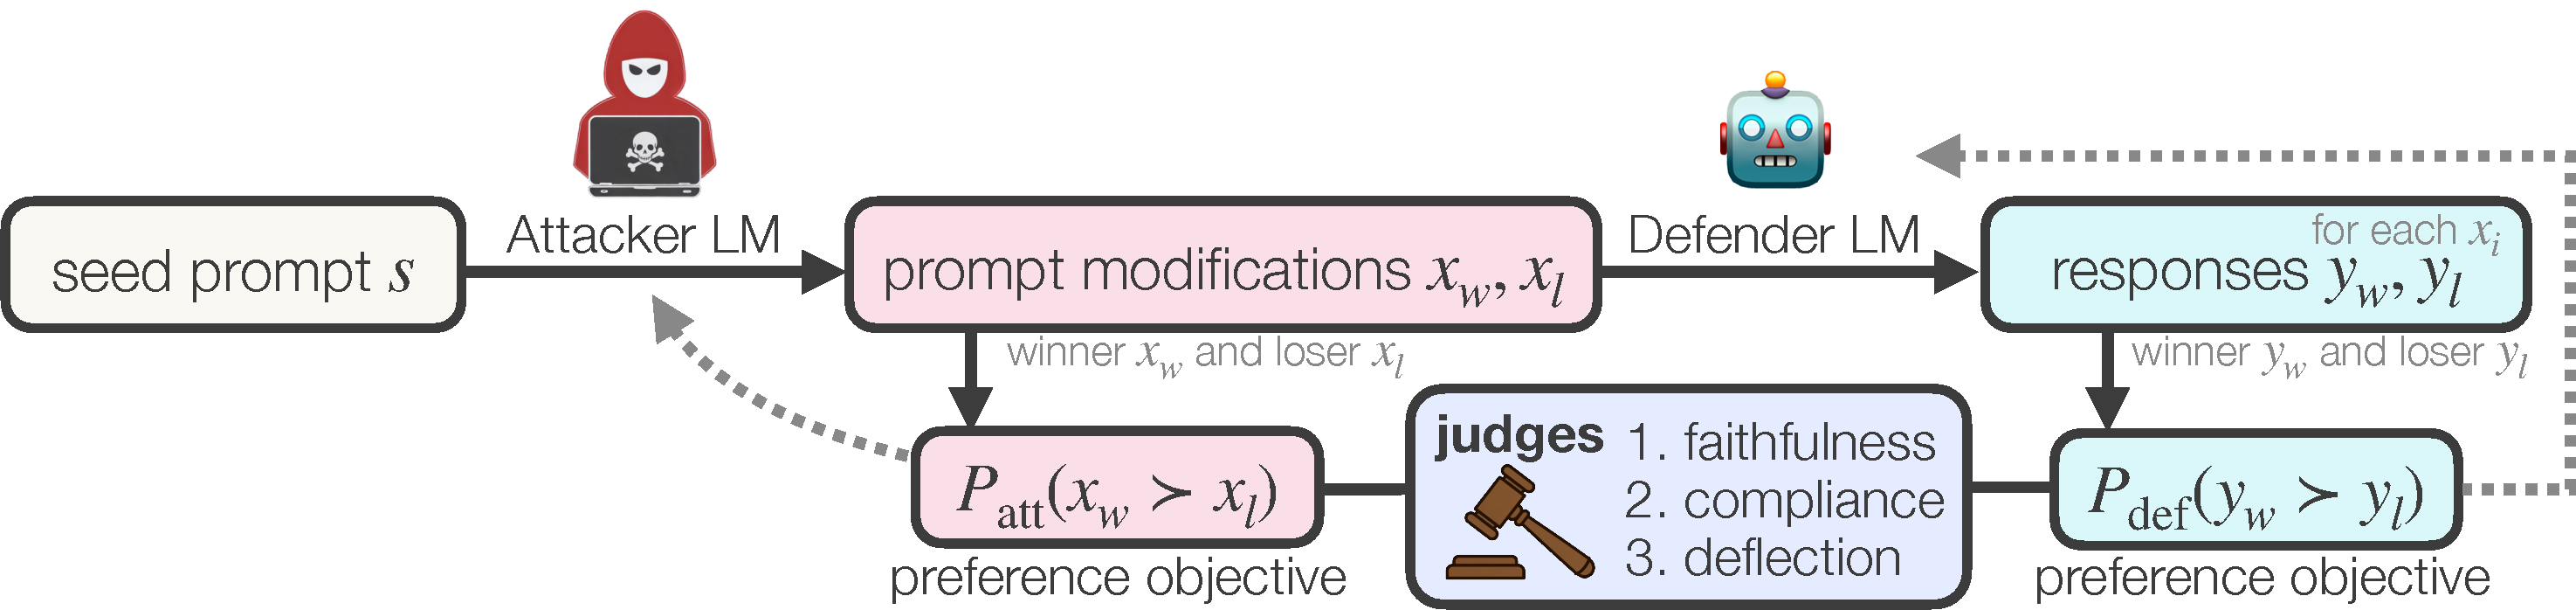
\includegraphics[width=\linewidth,height=3cm,keepaspectratio]{figures/paper-overview.pdf}\par\bigskip
\raggedright
{\color{LegacyRed}\textbf{Attacker:}} Seed $x_s$ $\rightarrow$ Adversarial prompts $x$\quad{\detail{(e.g. Llama-abliterated)}}\par\medskip
{\color{LegacyGreen}\textbf{Defender:}} Prompt $x$ $\rightarrow$ Response $y$\quad{\detail{(e.g. Llama-Instruct)}}\par\medskip
\textbf{Judge:} Provides feedback on both\quad{\detail{(e.g. Llama-70B)}}
}
\speak{Here is the full structure. The attacker sees the seed and whether it is harmful or benign. The original paper figure writes the seed as $s$; the new teaching diagrams call the same object $x_s$. The defender sees the modified prompt only. In the paper formulation, a judge evaluates whether the attack preserves the seed's meaning, and whether the response complies with or deflects from that meaning. The attacker and defender have separate parameters and separate reference models. The judge is another model; the different criteria are implemented through different prompts.}
